\documentclass[class=article, crop=false]{standalone}
\usepackage{mathtools}
\usepackage{amsmath}
\usepackage{float}
\usepackage{algorithmic}
\usepackage[ruled]{algorithm2e}
\setcounter{section}{0}
\usepackage[subpreambles=true]{standalone}
\usepackage{import}
\begin{document}
\section{Introduction}
Le Whale Optimization Algorithm est une nouvelle métaheuristique introduite en 2016 par Mirjalili et Lewis basée sur l’intelligence en essaim. Cet algorithme est inspiré d’une stratégie d’alimentation des baleines à bosse connue sous le nom de L'alimentation au filet à bulles. Une tactique qui leur permet d’attraper le plus de poissons possibles en un seul coup. Après avoir détecté ses proies, la baleine libère des bulles en nageant dans un mouvement spirale vers la surface pour encercler la proie pour la capturer.
Les bulles libérées peuvent prendre 2 formes : une forme de cercles rétrécissants \textbf{\emph{[figure 01]}} ou une forme spirale \textbf{\emph{[figure 02]}}. 
Dans cet algorithme, La recherche des proies représente l’exploration de l’espace de recherche et La libération des bulles représente l’exploitation.
\begin{figure}[H] 
    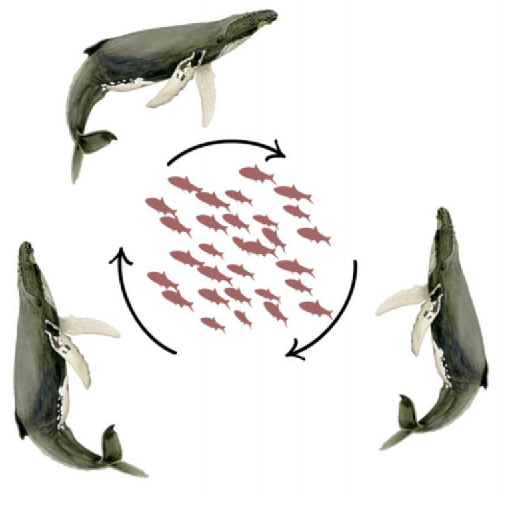
\includegraphics[width=\linewidth]{../figures/cercles.png}
    \caption{Libération des bulles en cercles rétrecissants}
\end{figure}

\begin{figure}[H] 
    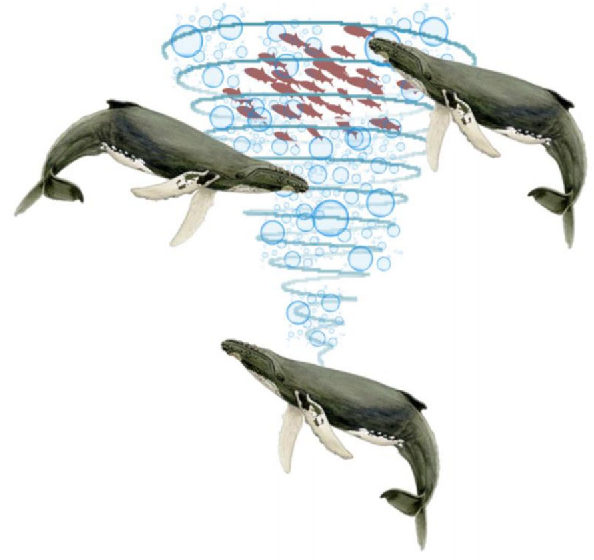
\includegraphics[width=\linewidth]{../figures/spiral.png}
    \caption{Libération des bulles en spirale}
\end{figure}

\section{Représentation mathématique :}
\subsection{Encerclement avec bulles en cercles rétrécissants :}
Soient:
\begin{itemize}
    \item \(x^*(t)\) la meilleure solution courante.
    \item \(t\) le numéro de l'itération courante.
    \item \(\vec{D}\) indique la distance du ième baleine (ième solution candidate) à la proie (la meilleure solution actuelle).
    \item \(x(t)\) une solution de la population à l'itération \(t\), et \(x(t+1)\) le résultat de sa mise à jour.
    \item \(x_r(t)\) une solution choisie aléatoirement de la la population courante.
    \item \(A\) et \(C\) des coefficients calculés par les formules suivantes:
    \[A = 2ar-a\] 
    \[C = 2r\] 
    Avec \(r\) un nombre aléatoire appartenant à \([0,1]\).
    \\ et \(a\) un nombre décrémenté linéairement à chaque itération de 2 à 0, de la façon suivante:
    \(a =  a_{init} - a_{init}*i/max\_iter\) avec \(i\) numéro de l’itération courante, \(max\_iter\) le nombre maximal des itération et \(a_{init}\) la valeur initiale de \(a\).
\end{itemize}
Le processus d’encerclement de la proie peut être représenté par les équations suivantes :

\begin{equation*}
    \vec{D} = |Cx^*(t) - x(t)|
\end{equation*}
Si \(|A| < 1\):
\begin{equation}
    x(t+1) = x^*(t) - A\vec{D}
\end{equation}
Sinon:
\begin{equation}
    x(t+1) = x_r(t) - A\vec{D}
\end{equation}
Le comportement de l’encerclement avec bulles en cercle rétrécissant est obtenu en diminuant la valeur de \(a\) de \(a_{init}\) à 0 au cours des itérations. La variation de \(A\) peut être utilisée pour rechercher des proies, c'est-à-dire la phase d'exploration. Par conséquent, \(A\) peut être utilisé avec des valeurs aléatoires supérieures à 1 ou inférieures à -1 pour forcer les solutions à s'éloigner de la solutions de référence (la meilleure solution \(|A| < 1\) ou une solution aléatoire sinon).
\subsection{Encerclement avec bulles sous forme spirale :}
Il est modélisé par les équations suivantes :
\begin{equation}
    \vec{D} = |x^*(t) - x(t)|
\end{equation}
\begin{equation}
    x(t+1) = \vec{D} e^{bl} \cos (2\pi l) + x^*(t)
\end{equation}
Où \(l\) est un nombre aléatoire appartenant à \([-1,1]\) Et \(b\) une constante qui définit la forme de la spirale 

Ces deux types définissent deux mécanismes d’explorations de l’espace recherche, ce qui permet une meilleure diversification de l’espace de recherche.
Dans chaque itération du WOA, un de ces deux mécanismes est choisi avec une probabilité \(p\) égale à \(50\%\) pour mettre à jour la population des solutions candidates comme suit:
\[ x(t+1) =
  \begin{cases}
    x^*(t) - A\vec{D}       & \quad r < p\\
    \vec{D} e^{bl} \cos (2\pi l) + x^*(t)  & \quad r \geq p
  \end{cases}
\]
avec \(x*(t)\) est la meilleure solution actuelle au temps \(t\), \(p\) est égal à \(0,5\) et \(r\) est un nombre aléatoire entre \([0, 1]\)

\subsection{Pseudocode:}
\begin{algorithm}[H]
    \SetAlgoLined
    \KwResult{Nombre de boîte utilisées.}
    Initialiser la population de baleines (l'ensemble initial des solutions candidates): Xi (i = 1, 2 ,..., N)\;
    Évaluer les solutions de la population initiale\;
    X* = la meilleure solution actuelle\;
    \While{\(t < max\_iter\)}{
        \For{solution \(\in\) population}{
            Mettre à jour a, A, C, l et r\;
            \eIf{\(r  < 0,5\)}{
                \eIf{\(|A| < 1\)}{
                    Mettre à jour la solution par Eq.(1)\;
                }{
                    Sélectionnez une solution aléatoire \(X_r\)\;
                    Mettre à jour la solution par Eq.(2)\;
                }
            }{
                Mettre à jour la solution par l'Eq.(4)\;
            }
        }
        Vérifier si une solution dans la population dépasse l'espace de recherche et la modifier\;
        Évaluer chaque solution\;
        Mettre à jour X* s'il existe une meilleure solution\;
        t = t + 1\;
     }
    \caption{Whale Optimization Algorithm}
    \end{algorithm}
\subsection{Ingrédients du WOA :}
\begin{itemize}
    \item Population initiale des solutions.
    \item Fonction d’évaluation qui permet de choisir la meilleure solution x*(t).
    \item Un mécanisme d'évolution:
    \begin{itemize}
        \item Encerclement avec bulles en cercle rétrécissant.
        \item Encerclement avec bulles sous forme de spirale.
    \end{itemize}
    \item Critère d'arrêt du WOA: nombre maximal d’itérations.    
\end{itemize}
\subsection{Paramètres du WOA :}
\begin{itemize}
    \item La taille de la population des solutions candidates à évaluer dans chaque itération.
    \item La constante \(b\) qui définit la forme de la spirale.
    \item Le nombre maximal d’itérations: \(max_iter\).
    \item le nombre \(a\) qui détermine le degré de diversification (exploration).    
\end{itemize}
\subsection{Application de l’algorithme au problème du bin packing :}
\subsubsection{Discrétisation de l'espace de recherche :}
Cet algorithme a été proposé pour la résolution de problèmes à espace \\ de recherche continu. Afin de l’adapter à notre problème discret nous allons utiliser une méthode appelée LOV qui permet de passer d’une solution continue à une solution discrète:\\
\begin{algorithm}[H]
    \SetAlgoLined
    \KwResult{Solution discrète \(X = (x_1, x_2, \dots, x_n)\) obtenue à partir de la solution continue \(\tilde{X} = (\tilde{x_1}, \tilde{x_2}, \dots, \tilde{x_n})\)}
    Ordonnez les valeurs du vecteur de \(\tilde{X}\) par ordre décroissant\;
    L'indice d'ordre de caque valeur est stocké dans un vecteur \(\theta = \{ \theta_i = \text{ordre de l'élément } \tilde{x_i}\}\)\;
     \caption{Discrétisation de l'espace de recherche par LOV}
    \end{algorithm}
\subsubsection{Représentation d’une solution :}
Une solution est exprimée par un vecteur \(x(t)=(a_1, a_2, …, a_n)\) représentant la distribution des articles dans les boîtes au moment t, avec n le nombre d’article et ai est un article d’ordre i. Les articles sont ordonnés selon les boîtes dans lesquelles ils sont rangés, i.e. l’article a1 est rangé dans la première boîte, s’il y’en a de l’espace dans cette boîte alors l’article a2 est y rangé, sinon a2 est rangé dan la deuxième boîte...ainsi de suite. ( principe du Next Fit) 
Une solution \(x(t)\) appartient au domaine de recherche tant qu’elle respecte les contraintes du problème: un objet ne peut pas être rangé dans plus d’une boîte, donc pas de doublons dans x(t), l’autre contrainte concernant le respect de la capacité d’une boîte est vérifié trivialement par définition du vecteur x(t).

\subsubsection{La fonction objectif :}
Afin de pouvoir évaluer les solutions, Nous avons opté pour la fonction suivante proposée par \emph{Hyde et al} [add ref here], au lieu du nombre de boîtes utilisées, parce que avec cette dernière pour plusieurs solutions on peut avoir la même évaluation ce qui peut engendrer la stagnation de l’algorithme.
\[ F_{min} = 1 - \frac{\sum_{1}^{n} (occup_i / c)^k}{n}\]
Avec:
\begin{itemize}
    \item \(n\) nombre de boites utilisées.
    \item \(ocup_i\) total des poids des objets rangés dans l’ième.
    \item \(c\) capacité des boites.
    
\end{itemize}
\end{document}